\appendix
% \appendixpage
% \addappheadtotoc
\section{Parabola of Revolution}
\label{app:parabola}

In this section we develop the particular case of the parabola.
The parametrization is given by:

\begin{align}
x &= - \frac{1}{2}R_ct^2 + R_0 \\
y &= R_c t
\end{align}
Where $R_c$ is the radius of curvature and $R_0$ is the distance of the parabola nose to the
origin.
The respective tridimensional shape is given by:
\begin{align}
x &= -\frac{1}{2}R_ct^2 + R_0 \label{eq:x-par-a}\\
y &= R_c t \cos\phi  \label{eq:y-par-a}\\
z &= R_c t \sin\phi  \label{eq:z-par-a}
\end{align}
The azimutal angle where the surface is tangent to the line of sight in this case is given by:
\begin{align}
\sin\phi_t = -\frac{\tan i}{t} \label{eq:sin-tan-a} 
\end{align}

Subtituting (\ref{eq:sin-tan-a}) into (\ref{eq:x-par-a}), (\ref{eq:y-par-a}) and
(\ref{eq:z-par-a}) we find the apparent shape
of the paraboloid:

\begin{align}
x' &= -\frac{R_c(\frac{1}{2}t^2 \cos^2 i -\sin^2 i)}{\cos i}+R_0\cos i \\
y' &= R_c\left(t^2-\tan^2 i\right)^{1/2} 
\end{align}

Taking the limit of equations (\ref{eq:qprime}) and (\ref{eq:Aprime}) when $\theta_c$ tends to zero we find that:

\begin{align}
\left(\frac{q'}{q}\right)_{\mathrm{parabola}} &= 1+\frac{\tilde{R}_c\tan^2 i}{2}\\
\left(\tilde{R}'_c\right)_{\mathrm{parabola}} &= \frac{\tilde{R}_c}{\cos^2 i + \frac{\tilde{R}_c}{2}\sin^2 i}
\end{align}

\section{Analytic derivation of the radius of curvature in the Thin Shell model}
\label{app:rc-analytic}

For small $\theta$ we may do a polynomial expansion for the shell shape such as:

\begin{align}
R \simeq R_0\left(1+\gamma\theta^2 + \Gamma\theta^4\right) \label{eq:R-exp}
\end{align}

The radius of curvature at the axis for $R$ is given by:

\begin{align}
R_c = R_0\left(1-2\gamma\right)^{-1}
\end{align}

The coefficient gamma may be derived by an expansion at small angles of equation
(\ref{eq:th1th}), as follows:

From the first term of the right side we get:

\begin{align}
\cot\theta &\simeq \theta^{-1}\left[1-\frac{1}{3}\theta^2\right] \\
\cos^k\theta\sin^2\theta &\simeq \theta^2 - \left(\frac{1}{3} + \frac{k}{2}\right)\theta^4 \\
\implies I_k(\theta) &\simeq \frac{1}{3}\theta^3\left[ 1 - \frac{1}{10}(3k+2)\theta^2\right]\\
\implies 2\beta I_k(\theta)\cot\theta &\simeq \frac{2}{3}\beta\theta^2\left[1-\frac{1}{30}
(9k+16)\theta^2\right]\label{eq:AR1} 
\end{align}

For the second term we get:

\begin{align}
-\frac{2\beta}{k+2}\left(1-\cos^{k+2}\theta\right) & \simeq -\beta\theta^2\left[1-\frac{1}{12}
(3k+4)\theta^2\right] \label{eq:AR2}
\end{align}

For the left side we use equation (25) from \CRW{}. Then, equation (\ref{eq:th1th}) results
as follows:

\begin{align}
\theta_1^2\left(1+\frac{1}{15}\theta_1^2\right) = \beta\theta^2\left[1+\frac{1}{60}(4-9k)
\theta^2\right] \label{eq:th1th-app}
\end{align}

And we can use the approximation $\theta_1 \approx \beta\theta^2$ for the correction term in
the left side of (\ref{eq:th1th-app}):

\begin{align}
\theta_1^2 &= \beta\theta^2\left[1+\frac{1}{60}(4-9k)\theta^2\right]
\left(1-\frac{\beta}{15}\theta^2\right) \\
\implies \theta_1^2 &= \beta\theta^2\left[1+ 2C_{k\beta}\theta^2\right]
\label{eq:th1th-small}\\
\mathrm{where:~} C_{k\beta} &\equiv \frac{1}{2}\left(A_k-\frac{\beta}{15}\right) \\
A_k &\equiv \frac{1}{15}-\frac{3k}{20}
\end{align}

Now, using equation (23) from \CRW{} we may estimate $R$ at low angles. To do this, we need to
expand each term as follows (neglecting terms of order four or higher):

\begin{align}
\theta_1 = &= \beta^{1/2}\theta\left[1+ 2C_{k\beta}\theta^2\right]^{1/2} \\
\theta + \theta_1 &= \theta\left[1+\beta^{1/2}\left(1+2C_{k\beta}\theta^2\right)\right]\\
\sin\theta_1 &= \theta_1\left[1-\frac{\theta_1^2}{6}\right] \\
 &= \beta^{1/2}\theta\left[1+\left(C_{k\beta}-\frac{1}{6}\beta\right)\theta^2\right] \\
 \sin(\theta+\theta_1) &= \left[\theta+\theta_1\right]\left[1-\frac{\left(\theta+\theta_1
 \right)^2}{6}\right] \\
 &= \theta\left(1+\beta^{1/2}\right)\left\lbrace 1+\left[\frac{C_{k\beta}\beta^{1/2}}
 {1+\beta^{1/2}}-\frac{1}{6}\left(1+\beta^{1/2}\right)^2\right]\theta^2\right\rbrace
\end{align}


So, combining these terms with equation (23) from \CRW{} we found the final expression for $R$:

\begin{align}
\frac{R}{D}\equiv \frac{\sin\theta_1}{\sin(\theta+\theta_1)} = \frac{\beta^1/2}{1+\beta^{1/2}}
\left\lbrace 1 + \theta^2\left[\frac{C_{k\beta}}{1+\beta^{1/2}}+\frac{1}{6}\left(1+2\beta^{1/2}
\right)\right] \right\rbrace \label{eq:r-small-theta}
\end{align}

Returning to equation (\ref{eq:R-exp}) we see the following:

\begin{align}
R_0 &= \frac{\beta^{1/2}}{1+\beta^{1/2}} \\
\gamma &= \frac{C_{k\beta}}{1+\beta^{1/2}}+\frac{1}{6}\left(1+2\beta^{1/2}\right)
\label{eq:app-gamma}
\end{align}

We recover equation (27) of \CRW{} for $R_0$ and equation (\ref{eq:app-gamma}) is the
needed term to calculate the radius of curvature at the axis.

\section{Analytic derivation of \texorpdfstring{\boldmath $R_{90}$}{R\_90} in the thin shell model}
\label{app:r90-analytic}

To derive $R_{90}$ we need to evaluate equations (23) from \CRW{} and (\ref{eq:th1th})
at $\theta=\frac{\pi}{2}$:

\begin{align}
R_{90} = D\tan\theta_{1,90} \\
\theta_{1,90}\cot\theta_{1,90} -1 = -\frac{2\beta}{k+2} \label{eq:th190}
\end{align}
Where $\theta_{1,90}\equiv \theta_1(\frac{\pi}{2})$. Combining both equations and  introducing
the parameter $\xi\equiv \frac{2}{k+2}$ we have:
\begin{align}
R_{90} &= D\frac{\theta_{1,90}}{1-\xi\beta} \label{eq:r90-incomplete}
\end{align}

Expanding the left side of (\ref{eq:th190}) until fourth order, equation (\ref{eq:th190})
becomes:

\begin{align}
\theta_{1,90}^2\left(1+\frac{\theta_{1,90}^2}{15}\right) \simeq 3\xi\beta
\end{align}

Applying the approximation $\theta_1^2 \approx 3\xi\beta$ we found a solution
for $\theta_{1,90}$:

\begin{align}
\theta_{1,90} = \left(\frac{3\xi\beta}{1+\frac{1}{5}\xi\beta}\right)^{1/2}
\end{align}

And substituting into (\ref{eq:r90-incomplete}) we find the solution for $R_{90}$:

\begin{align}
R_{90} &= \frac{\left(3\xi\beta\right)^{1/2}}{\left(1+\frac{1}{5}\xi\beta\right)^{1/2}
\left(1-\xi\beta\right)} \\
\implies \tilde{R}_{90} &\equiv \frac{R_{90}}{R_0} = \frac{\sqrt{3\xi}\left(1+\beta^{1/2}\right)}
{\left(1+\frac{1}{5}\xi\beta\right)^{1/2}\left(1-\xi\beta\right)}
\end{align}

\section{Derivation of Characteristic Radii in Isotropic Wind/Parallel interaction Problem}
\label{app:ch-rad-Wilkin}

$\tilde{R}_{90}$ is obtained by simply evaluating equation (\ref{eq:R-Wilkin}) at $\theta=\frac{\pi}{2}$.
For the Radius of curvature we follow a similar procedure than the Wind/Wind interaction, but using equation
(\ref{eq:R-Wilkin}) for $R(\theta)$ and inserting the cosecant into the square root.

Expanding the terms of $R(\theta)$ we find the following:

\begin{align}
  \csc^2\theta &\simeq \theta^{-2}\left[1+\frac{\theta^2}{3}\left(1+\frac{\theta^2}{5}\right)\right] \\
  1-\theta\cot\theta &\simeq \frac{\theta^2}{3}\left[1 + \frac{\theta^2}{15}\left(1+\frac{2\theta^2}{21}\right)\right] \\
  \implies \tilde{R}(\theta) \simeq 1 + \frac{\theta^2}{5} + O\left[\theta^4\right]
\end{align}

From equation (\ref{eq:Rcurv}) for the radius of curvature we finally get the numerical value for $\tilde{R_c} = \frac{5}{3}$

\section{Distribution of p-values for all correlations tested}
\label{sec:distr-p-values}

\begin{figure}
  (a)\\
  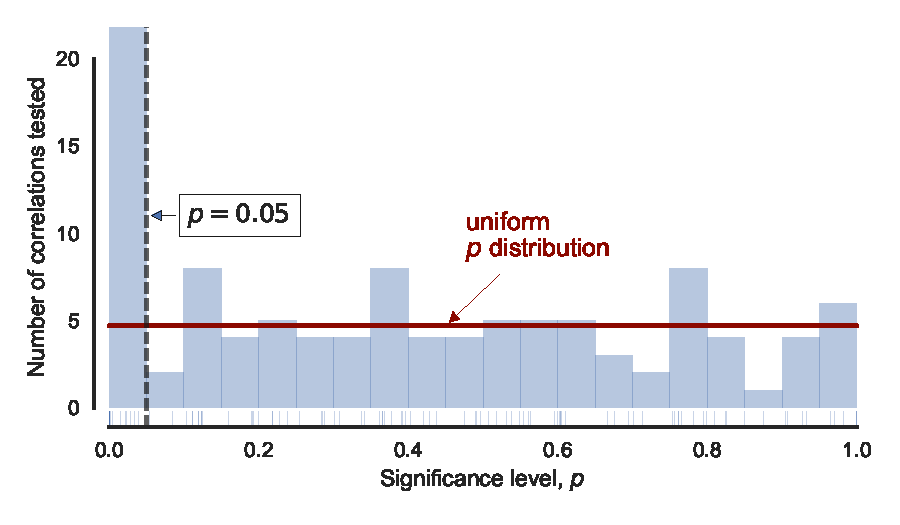
\includegraphics[width=\linewidth]{figs/p-value-histogram-new-linear}\\
  (b)\\
  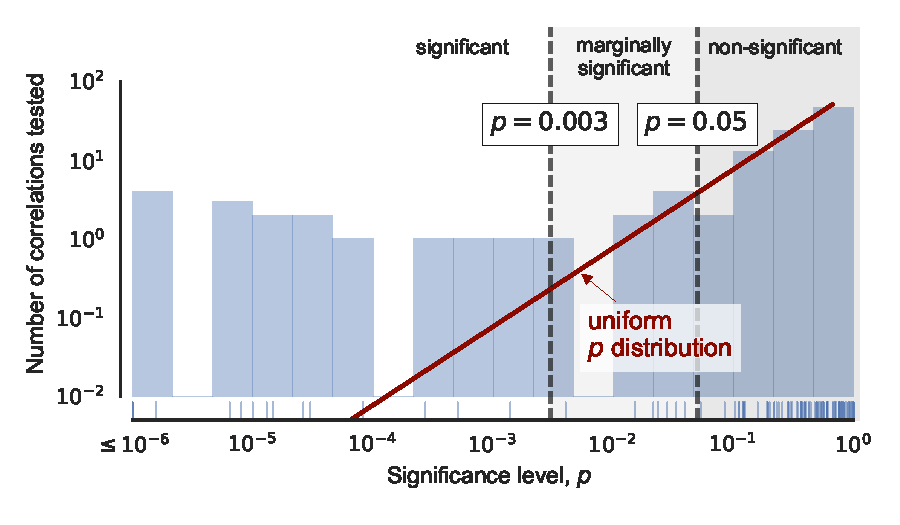
\includegraphics[width=\linewidth]{figs/p-value-histogram-new}
  \caption{Histogram of \(p\)-values for all non-parametric 2-sample
    tests performed during the analysis of
    section~\ref{sec:comp-with-observ}. (a)~Uniformly spaced linear
    bins and linear vertical axis. (b)~Uniformly spaced logarithmic
    bins and logarithmic vertical axis, with all values
    \(p \le 10^{-6}\) included in the leftmost bin.  The vertical dashed
    lines shows the traditional threshold values for significance:
    \(p = 0.001\) and \(p = 0.05\). The red solid line shows the
    uniform distribution of \(p\)-values that would be expected if the
    null hypothesis were always true, that is, if no significant
    correlations existed.}
  \label{fig:histo-p-values}
\end{figure}


\begin{table}
  \caption{Lower bounds on the Type~I error rate, \(\alpha\)}
  \label{tab:type-I}
  \centering
  \begin{tabular}{lrr} \toprule
    Correlation & \(p\) & \(\alpha\) \\
    \midrule
    \multicolumn{3}{l}{\itshape Quantitative \dotfill}\\
    \(R_c\) vs \(R_0\) & \textit{0.0054} & \textit{0.0712} \\
    \(R_{90}\) vs \(R_0\) & \textbf{0.0001} & \textbf{0.0025} \\
    \(R_c\) vs \(H_0\) & 0.1229 & 0.4119 \\
    \(R_{90}\) vs \(H_0\) & \textit{0.0215} & \textit{0.1833} \\
    \(R_c\) vs \(A_K\) & 0.19 & 0.4617 \\
    \(R_{90}\) vs \(A_K\) & 0.63 & 1 \\
    \(R_c\) vs \(|b|\) & 0.19 & 0.4617 \\
    \(R_{90}\) vs \(|b|\) & 0.31 & 0.4967 \\
    \(R_c\) vs \(\cos(\ell)\) & 1.00 & 1 \\
    \(R_{90}\) vs \(\cos(\ell)\) & 0.36 & 0.4999 \\
    \midrule
    \multicolumn{3}{l}{\itshape Categorical} \dotfill\\
    \(R_c\) vs Facing & 0.71 & 1 \\
    \(R_c\) vs H II & 0.50 & 1 \\
    \(R_{90}\) vs Facing & 0.60 & 1 \\
    \(R_{90}\) vs H II & 0.52 & 1 \\
    \(R_c\) vs Multiple & 1.00 & 1 \\
    \(R_{90}\) vs Multiple & 0.34 & 0.4993 \\
    \(R_c\) vs \SI{8}{\um} & 0.82 & 1 \\
    \(R_{90}\) vs \SI{8}{\um} & 0.6 & 1 \\
    \midrule
    \multicolumn{3}{l}{\itshape Other datasets} \dotfill\\
    \(R_c\) vs Herschel & 0.074 & 0.3437 \\
    \(R_{90}\) vs Herschel & \textbf{0.00052} & \textbf{0.0106} \\
    \(R_c\) vs M42 & \textbf{0.00048} & \textbf{0.0099} \\
    \(R_{90}\) vs M42 & \textbf{0.0000105} & \textbf{0.0003} \\
    \bottomrule
  \end{tabular}
\end{table}


The \(p\)-values are the probability of finding a difference between
two populations as large as (or larger than) what is observed,
\emph{given} that there is no difference in the underlying
distribution from which the two populations are drawn (that is, given
that the null hypothesis is true).  However, what we really want to
know is something else: the probability that the null hypothesis is
true, \emph{given} the observations.  That is, the probability,
\(\alpha\), of a \textit{false positive}, also known as the \textit{Type I
  error rate}.  The common mistake of conflating these two definitions
is known as the ``\(p\)-value fallacy'' \citep{Goodman:1999a}, or``the
error of the transposed conditional'', as discussed in detail by
\citet{Colquhoun:2014a}.  It is possible to derive \(\alpha\) from
\(p\) using Bayes' theorem (e.g., \citealp{Goodman:1999b}), but that
requires an estimate of the prior probability of the null hypothesis,
independent of the observations.  Alternatively, it is also possible
to find a lower bound on \(\alpha\) from a frequentist approach
\citep{Sellke:2001a}:
\begin{equation}
  \label{eq:type-I}
  \alpha(p) \ge \bigg[ 1 - \big(e\, p \ln p\big)^{-1} \bigg]^{-1}
  \quad \text{valid for } p < 1/e.
\end{equation}
This is the approach we adopt here, which also numerically coincides
with the Bayesian approach for the case where the prior probability of
the null hypothesis is 0.5.  The reason that this is only a lower
limit for \(\alpha\) is that if we have overwhelming a priori evidence that
the null hypothesis is true (for instance, from previous empirical
studies, or because it follows from a well-supported theory), then a
Bayesian calculation would give a much higher value of \(\alpha\) than
\eqref{eq:type-I} does.  In our case, however, we have no strong
reasons for favoring any of the null hypotheses, so it is reasonable
to assume \(\alpha\) is close to the lower limit given in \eqref{eq:type-I}.

In order to choose a threshold \(p\)-value that counts as a
``significant'' result, one then needs to balance the risks of false
positives against the risks of \textit{false negatives}.  The false
negative probability, \(\beta\), also known as \textit{Type II error
  rate}, is the probability of failing to reject an untrue null
hypothesis.  That is, in the context of this paper, it is the
probability of failing to detect a real difference between two
sub-samples, or a real correlation between two variables.  The
complementary probability, \(1 - \beta\), is known as the
\textit{statistical power} or sensitivity of the test.  The value of
\(\beta\) depends on three factors:
\begin{enumerate}[1.]
\item The \textit{effect size}, which is a measure of the magnitude of
  the difference in a dependent variable between two sub-samples, or
  the degree of correlation between two continuous variables.  For the
  two sub-sample case, it is common to use a standardised mean
  difference, such as Cohen's \(d\) statistic \citep{Cohen:1988a}:
  \(d = (\bar{X}_A - \bar{X}_B) / s\), where \(\bar{X}_A\),
  \(\bar{X}_B\) are the means of the dependent variable \(X\) for
  samples A and B, while \(s\) is the pooled standard deviation of
  \(X\).  For the case of two continuous variables, the Pearson linear
  correlation coefficient, \(r\), can be used.  In both cases, rules
  of thumb have been developed \citep{Ruscio:2008a} for classifying an
  effect as ``large'' (\(d > 0.8\), \(r > 0.4\)) or ``small''
  (\(d < 0.2\), \(r < 0.1\)).  Alternatively, non-parametric
  statistics can be used, such as the \(A\) measure of stochastic
  superiority \citep{Delaney:2002a}.
\end{enumerate}

Obviously, this depends on the \textit{effect size}, which is the 


All astronomical data analysis is \emph{post hoc} analysis, since the universe was not set up to test a particular hypothesis (as far as we know).  It is therefore important to guard against the ``multiple comparisons problem'', whereby seemingly significant correlations are found where none really exist, simply by virtue of the large number of tests that were carried out.

Under the more conservative Holm--Bonferroni method, only comparisons with \(p < 0.001\) would be significant. 

The p-curve \citep{Head:2015a}

%%% Local Variables:
%%% mode: latex
%%% TeX-master: "quadrics-bowshock.tex"
%%% End:
